\chapter{CHAPTER FOUR: RESULTS} \label{chapter_4}


\begin{figure}[!ht] \singlespacing
\begin{center}
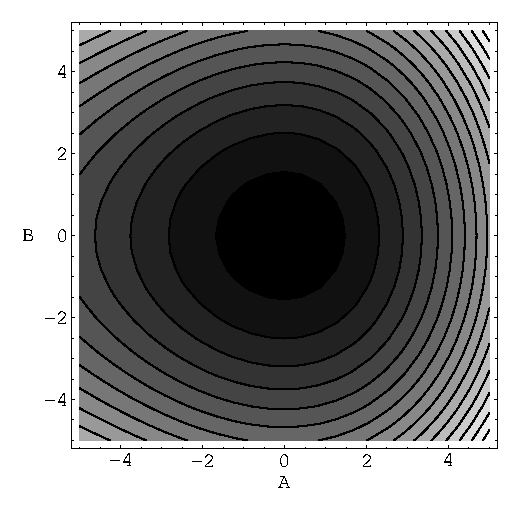
\includegraphics[width=.8\textwidth]{figures/homoclinic}  %% good idea to keep your figures in a separate folder
\end{center}
\caption{Homoclinic Orbit}\label{tbl:my_first_figure}
\end{figure}

%% Best way to generate pictures, especially graphs, is to save them (say from MATLB) as .eps (Encapsulated PostScript) and than
%% convert to PDF using (attached) eps2pdf utility. Note that pdfTeX will not accept .eps files.
